\documentclass{article}[18pt]
\ProvidesPackage{format}
%Page setup
\usepackage[utf8]{inputenc}
\usepackage[margin=0.7in]{geometry}
\usepackage{parselines} 
\usepackage[english]{babel}
\usepackage{fancyhdr}
\usepackage{titlesec}
\hyphenpenalty=10000

\pagestyle{fancy}
\fancyhf{}
\rhead{Sam Robbins}
\rfoot{Page \thepage}

%Characters
\usepackage{amsmath}
\usepackage{amssymb}
\usepackage{gensymb}
\newcommand{\R}{\mathbb{R}}

%Diagrams
\usepackage{pgfplots}
\usepackage{graphicx}
\usepackage{tabularx}
\usepackage{relsize}
\pgfplotsset{width=10cm,compat=1.9}
\usepackage{float}

%Length Setting
\titlespacing\section{0pt}{14pt plus 4pt minus 2pt}{0pt plus 2pt minus 2pt}
\newlength\tindent
\setlength{\tindent}{\parindent}
\setlength{\parindent}{0pt}
\renewcommand{\indent}{\hspace*{\tindent}}

%Programming Font
\usepackage{courier}
\usepackage{listings}
\usepackage{pxfonts}

%Lists
\usepackage{enumerate}
\usepackage{enumitem}

% Networks Macro
\usepackage{tikz}


% Commands for files converted using pandoc
\providecommand{\tightlist}{%
	\setlength{\itemsep}{0pt}\setlength{\parskip}{0pt}}
\usepackage{hyperref}

% Get nice commands for floor and ceil
\usepackage{mathtools}
\DeclarePairedDelimiter{\ceil}{\lceil}{\rceil}
\DeclarePairedDelimiter{\floor}{\lfloor}{\rfloor}

% Allow itemize to go up to 20 levels deep (just change the number if you need more you madman)
\usepackage{enumitem}
\setlistdepth{20}
\renewlist{itemize}{itemize}{20}

% initially, use dots for all levels
\setlist[itemize]{label=$\cdot$}

% customize the first 3 levels
\setlist[itemize,1]{label=\textbullet}
\setlist[itemize,2]{label=--}
\setlist[itemize,3]{label=*}

% Definition and Important Stuff
% Important stuff
\usepackage[framemethod=TikZ]{mdframed}

\newcounter{theo}[section]\setcounter{theo}{0}
\renewcommand{\thetheo}{\arabic{section}.\arabic{theo}}
\newenvironment{important}[1][]{%
	\refstepcounter{theo}%
	\ifstrempty{#1}%
	{\mdfsetup{%
			frametitle={%
				\tikz[baseline=(current bounding box.east),outer sep=0pt]
				\node[anchor=east,rectangle,fill=red!50]
				{\strut Important};}}
	}%
	{\mdfsetup{%
			frametitle={%
				\tikz[baseline=(current bounding box.east),outer sep=0pt]
				\node[anchor=east,rectangle,fill=red!50]
				{\strut Important:~#1};}}%
	}%
	\mdfsetup{innertopmargin=10pt,linecolor=red!50,%
		linewidth=2pt,topline=true,%
		frametitleaboveskip=\dimexpr-\ht\strutbox\relax
	}
	\begin{mdframed}[]\relax%
		\centering
		}{\end{mdframed}}



\newcounter{lem}[section]\setcounter{lem}{0}
\renewcommand{\thelem}{\arabic{section}.\arabic{lem}}
\newenvironment{defin}[1][]{%
	\refstepcounter{lem}%
	\ifstrempty{#1}%
	{\mdfsetup{%
			frametitle={%
				\tikz[baseline=(current bounding box.east),outer sep=0pt]
				\node[anchor=east,rectangle,fill=blue!20]
				{\strut Definition};}}
	}%
	{\mdfsetup{%
			frametitle={%
				\tikz[baseline=(current bounding box.east),outer sep=0pt]
				\node[anchor=east,rectangle,fill=blue!20]
				{\strut Definition:~#1};}}%
	}%
	\mdfsetup{innertopmargin=10pt,linecolor=blue!20,%
		linewidth=2pt,topline=true,%
		frametitleaboveskip=\dimexpr-\ht\strutbox\relax
	}
	\begin{mdframed}[]\relax%
		\centering
		}{\end{mdframed}}
\lhead{Software Engineering - HCI}


\begin{document}
\begin{center}
\underline{\huge HCI 1}
\end{center}
\section{Generations of computers}
\begin{enumerate}
	\item Vacuum tube (punchcards)
	\item Transistor (assembler language)
	\item Monitors, bytecode
\end{enumerate}
\section{HCI}
\begin{defin}[HCI]
The discipline concerned with the design, evaluation and implementation of interactive computer systems for human use and with the study of major phenomena surrounding them
\end{defin}
Objectives of HCI are
\begin{itemize}
	\item To provide an understanding of both the human user and the computer system, in an effort to make interactions between the two easier and more satisfying
	\item However the emphasis should always be on the user
\end{itemize}
\textbf{User}
\begin{itemize}
	\item An individual user, a group of users working together or a sequence of users in an organisation dealing with some part of a process or task
\end{itemize}
\textbf{Computer}
\begin{itemize}
	\item Technology ranging from desktop to large scale systems, or control/embedded systems
\end{itemize}
\textbf{Interaction}
\begin{itemize}
	\item Communication between the user and computer in a direct or indirect manner
\end{itemize}
\section{What is involved}
\begin{itemize}
	\item Study of humans using interfaces
	\item Development of new applications/systems to support user's activities
	\item Development of new devices and tools for users
	\item Develop usable products
	\begin{itemize}
		\item Easy to learn
		\item Effective to use
		\item Provide an enjoyable/satisfying experience
	\end{itemize}
\end{itemize}
\section{Why should you be concerned with HCI}
Increasingly becomes a matter of law\\
\\
National health ans safety standards constrain employers to provide their workforce with usable computer systems\\
\\
EC directive 90/270/EEC - when designing, selecting, commissioning or modifying software
\begin{itemize}
	\item Is suitable to task
	\item Is easy to use and adaptable to the user's knowledge and experience
	\item It provides feedback on performance
	\item It displays information in a format and at a pace that is adapted to the user
	\item It conforms to the "principle of software ergonomics"
\end{itemize}
Designers and employers cannot afford to ignore the user
\section{Principles for supporting HCI}
\begin{itemize}
	\item Listening to what people want and getting them involved in design
	\item Using tried and tested user-based techniques during the design process
	\item Thinking through what might provide quality user experiences
	\item Considering what might help people with the way they currently do things
	\item Taking into account what people are good and bad at
\end{itemize}
\section{Avoiding problematic design}
Take into account
\begin{itemize}
	\item Who the users are
	\item What activities are being carried out
	\item Where the interaction is taking place
\end{itemize}
\section{Memory and mental models}
\subsection{Multi-store memory}
Sensory memory
\begin{itemize}
	\item Iconic, Echoic, Haptic
	\item Hold info for a few tenths
	\item Attention passes info to short term memory
\end{itemize}
Short term memory store
\begin{itemize}
	\item Scratch pad for temporary recall of info
	\item Holds info for a few seconds (then decays)
	\item Has limited capacity 7+-2 digits for information
	\item Passed to long term memory via rehearsal 
\end{itemize}
Permanent long-term memory store
\begin{itemize}
	\item Everything we "know"
	\item Factual knowledge
	\item Experimental knowledge
	\item Procedural rules of behaviour etc.
	\item Hold information "indefinitely"
	\item Episodic - memory of events and experience in serial form
	\item Semantic - uses structure to store information derived from episodic memory list
\end{itemize}
\subsection{Mental models}
An explanation in what someone's though process for how something works in the real world\\
\\
A mental model is what the user believes about the system at hand\\
\\
Knowledge is sometimes described as a mental model
\begin{itemize}
	\item How to use the system (what to do next)
	\item What to do with unfamiliar systems or unexpected situations (how the system works)
\end{itemize}
People make inferences using mental models of how to carry out tasks
\begin{center}
	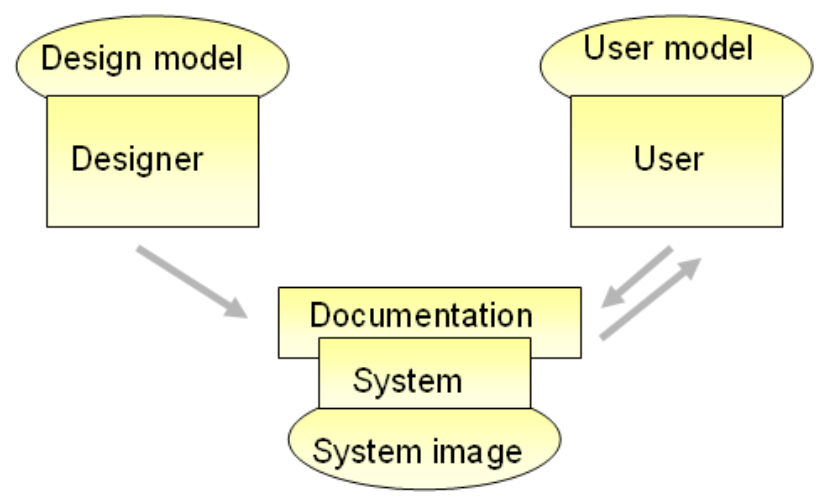
\includegraphics[scale=0.7]{Conceptual}
\end{center}
\subsection{What to do in HCI design}
Educate the user to build correct mental models\\
\\
Transparency:
\begin{itemize}
	\item Useful feedback in response to user input
	\item Easy to understand and intuitive ways of interacting with the system
	\item Provide the right kind and level of info in the form of:
	\begin{itemize}
		\item Clear and easy to follow instructions
		\item Appropriate online help and tutorials
		\item Context sensitive guidance for users, set at their level of experience 
	\end{itemize}
\end{itemize}
\section{HCI, science or craft?}
Both - artistically pleasing and capable of fulfilling the tasks required
\section{Cognition}
\begin{defin}[Cognition]
The process of acquiring knowledge through our thoughts, experiences and senses
\end{defin}
Cognition has also been described in terms of specific kinds of processes, including:
\begin{itemize}
	\item Attention - The process of selecting things to concentrate on
	\item Perception - How information is acquired from the environment
	\item Memory - Recalling various kinds of knowledge to allows appropriate actions
	\item Learning - How to use the computer based application or the use of a user based application to learn a topic
	\item Reading, speaking and listening - issues of information transience, speed etc
\end{itemize}
\subsection{Why do we need to understand users?}
\begin{itemize}
	\item Interacting with technology is cognitive
	\item Need to take into account cognitive process involved and cognitive limitations of users
	\item Provides knowledge about what users can and cannot be expected to do
	\item Identifies and explains the nature and causes of problems users encounter
\end{itemize}
\subsection{Attention}
Selecting things to concentrate on at a point in time from the mass of stimuli around us\\
\\
Allows us to focus on information that is relevant to what we're doing\\
\\
Involves audio and/or visual senses\\
\\
Focussed and divided attention enables us to be selective in terms of the mass of competing stimuli but limits our ability to keep track of all events\\
\\
Information at the interface should be structured to capture users' attention, e.g. use perceptual boundaries (windows), colour, sound and flashing lights
\subsubsection{Design implications for attention}
\begin{itemize}
	\item Make information salient when it needs attending to
	\item Use techniques that make things stand out like colour, ordering, spacing, underlining, sequencing and animation
	\item Avoid cluttering the interface with too much information
	\item Avoid using too much because the software allows it
\end{itemize}
\subsection{Gestalt Laws}
\textbf{Similarity} - Two visual stimuli that have a common property are seen as belonging together\\
\\
\textbf{Proximity} - Two visual stimuli that are close to each other are seen as belonging together\\
\\
\textbf{Closure} - If a set of stimuli almost encloses an area or could be interpreted as enclosing an area, the viewer sees the area\\
\\
\textbf{Good-Continuation} - Given a juncture of lines, the viewer sees as continuous those lines that are smoothly connected

\subsection{Perception}
How information is acquired from the environment via our senses\\
\\
Obvious implication is to design representations that are readily perceivable e.g.
\begin{itemize}
	\item Icons should be easy to distinguish and read
	\item Sounds or synthesized speech distinguishable
	\item Touch sensation - tactile feedback
	\item Visual groupings can help
	\item Text should be legible
\end{itemize}
\subsubsection{Design implications for Perception}
\begin{itemize}
	\item Use icons and other graphical representations; will enable users to easily recognise their meaning
	\item Bordering and spacing effective at grouping and finding info
	\item Sounds should be audible and distinguishable
	\item Text should be legible and distinguishable from the background
	\item Tactile feedback should allow users ti recognise and distinguish different meanings
\end{itemize}
\subsection{Memory}
\begin{itemize}
	\item Involves first encoding then retrieving knowledge
	\item We don't remember everything - involves filtering and processing what is attended to
	\item Context is important in affecting our memory - affects the extent to which info can be subsequently retrieved
	\item We recognise things much better than being able to recall things
\end{itemize}
\subsubsection{Recognition vs Recall}
\begin{itemize}
	\item Command based interfaced require users to recall from memory a name from 100s
	\item GUIs provide a visual way of doing the same
	\item Web browsers etc provide lists of visited URLs etch that support recognition in memory
\end{itemize}
\subsubsection{Digital content management}
Is a growing problem for many users:
\begin{itemize}
	\item Vast number of files of different types
	\item Where and how to save them all, then remembering what they were called and where to find them again
	\item Naming most common way of encoding them
	\item But can be difficult to remember, especially when we have 1000s and 1000s
	\item How might such a process be facilitated taking into account people's memory abilities?
\end{itemize}
\subsubsection{Design implications for Memory}
\begin{itemize}
	\item Do not overload users' memories with complicated procedures for carrying out tasks
	\item Design interfaces that promote recognition rather than recall by using menus, icons and consistently placed objects
	\item Provide users with a variety of ways to encode digital information to help them remember where they have stored them
\end{itemize}

\end{document}